\documentclass[letterpaper,11pt]{article}

%packages
\usepackage{amsfonts}
\usepackage{graphicx}
\usepackage[left=2cm,top=2cm,right=2cm,bottom=1.5cm,head=.5cm,foot=.5cm]{geometry}
\usepackage{url}
\usepackage{multirow}
\usepackage{longtable}
\usepackage{subfig}
\usepackage{float}
\usepackage{setspace}
\usepackage{lineno}
\usepackage{natbib}
\usepackage{amsmath}
\usepackage{authblk}
\usepackage{xr}
\usepackage{relsize}
\usepackage{tikz}
\usepackage{hyperref}

%new commands and so on
\providecommand{\keywords}[1]
{
  \small	
  \textbf{\textit{Keywords---}} #1
}

\DeclareMathOperator{\E}{\mathbb{E}}% expected value
\DeclareMathOperator{\var}{var}
\DeclareMathOperator{\cov}{cov}
\DeclareMathOperator{\cor}{cor}
\DeclareMathOperator{\mean}{mean}
\DeclareMathOperator{\se}{se}
\DeclareMathOperator{\sd}{sd}
\DeclareMathOperator{\prob}{P}

%attempt 1 at nat and sharp
%\newcommand{\nat}{\mathlarger{\natural}}
%\newcommand{\shp}{\mathlarger{\sharp}}

%attempt 2 at nat and sharp
%\newcommand{\nat}{\raisebox{1pt}{\mathsmaller{\mathsmaller{/\hspace{-2pt}/}}}}
%\newcommand{\shp}{\#}

%attempt 3 at nat and sharp
\newcommand{\nat}{%
\text{\hspace{-1.5pt}
\begin{tikzpicture}[scale=1.8]%
\draw (.333ex,0) -- (.333ex,1ex);%
\draw (.666ex,0) -- (.666ex,1ex);
\end{tikzpicture}%
}}
\newcommand{\shp}{%
\text{\hspace{-1.5pt}
\begin{tikzpicture}[scale=1.8]%
\draw (0,.333ex) -- (1ex,.333ex);%
\draw (0,.666ex) -- (1ex,.666ex);%
\draw (.333ex,0) -- (.333ex,1ex);%
\draw (.666ex,0) -- (.666ex,1ex);
\end{tikzpicture}%
}}
\newcommand{\test}{%
\text{
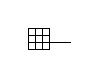
\begin{tikzpicture}[scale=1.8]%
\draw (0,0) -- (1ex,0ex);
\draw (0,0) -- (0ex,1ex);
\draw (0,1ex) -- (1ex,1ex);
\draw (1ex,0) -- (1ex,1ex);
\draw (0,.333ex) -- (2ex,.333ex);%
\draw (0,.666ex) -- (1ex,.666ex);%
\draw (.333ex,0) -- (.333ex,1ex);%
\draw (.666ex,0) -- (.666ex,1ex);
\end{tikzpicture}%
}}

\newcommand{\olr}{\overline{r}}
\newcommand{\olrs}{\overline{r}^{\shp}}
\newcommand{\olrn}{\overline{r}^{\nat}}
\newcommand{\bs}{\backslash}
\newcommand{\olep}{\overline{\epsilon}}

%header material for paper
\title{Responses to referees for ``Asymmetric relationships and their effects on coexistence''}
\date{September 2023}

\begin{document}

\noindent \emph{Dear Editors,} \\

\noindent \emph{Thank you for the useful and very positive reviews of our manuscript, and for
the opportunity to resubmit a revised version. We have addressed all referee comments below and in
the manuscript, and hope the paper can now be rapidly accepted. } \\

\noindent \emph{We have replied to referee comments below in italic, with each response preceded
by ``***'', to make our responses easier to find. We submit the following pdf files: The main text pdf, including all figures; 
the Supporting Information; and a version of the main text with changes tracked. The document showing 
the changes we made does not include links such as citations and
references to figures, but it does accurately represent the changes made to the text.} \\

\noindent \emph{We again thank the referees and editors for their feedback and positive reviews!} \\

\noindent \emph{Yours,}

\noindent \emph{Dan Reuman and Jasmin Albert} \\
%DONE with cover letter

\noindent \textbf{Comments of referee 1:} \\

\noindent C1) Thank-you to the authors for their response to my comments.

\noindent ***\emph{We appreciate your feedback which helped to improve our manuscript; thank you.} \\

\noindent C2) I have two minor suggestions remaining which I think should be straightforward to implement.

First, to consider introducing a discussion of the robustness to more esoteric definitions of the partial-sharp distributions, and adding this briefly to the main text.  Primarily as the authors already suggest in their response letter, as a signpost for future work.\\

\noindent ***\emph{} \\
%%JAS: added a sentence at the end of first paragraph of discussion. 

\noindent C3) The only other minor suggestion is that the authors clarify that in Fig 1 they are simply showing that ATAs do occur in nature.  I was not suggesting that the authors include examples pertinent to their question in Figure 1---as they say, readers may not be expecting this. I don't think that the connection between the ATAs in Fig 1 and the rest of the project are that clear, as I already expressed. But I respect the authors wishes (and their other feedback) that it is worthwhile including these. Just a sentence or so at some point explaining that these are not directly related to the ATAs relevant in the remainder of the paper may avoid confusion. \\

\noindent ***\emph{} \\
%%JAS: is it okay to put this is the caption of fig 1?
%%or in main, "Though not directly related to our questions at hand, 
%and for illustrative purposes, Fig1d,e show ... 

\noindent \textbf{Comments of referee 2:} \\

\noindent C4) This is a novel contribution highlighting that asymmetric tail associations in correlations between two variables was a very simple aspect not properly considered before but with huge implications for the maintenance of biodiversity. I congratulate the authors for their work. \\

\noindent ***\emph{Thank you for the very positive feedback and previous comments which helped to improve our manuscript!} \\
%DONE

\noindent \textbf{Comments of referee 3:} \\

\noindent C5) I thank the authors for the change and the nice discussion/replies to my questions. I especially like the new figure 2 which greatly helped my understanding of how to remove ATA. \\
  
\noindent ***\emph{Many thanks for the positive feedback which improved our manuscript to become more understandle to other readers as well!} \\

\noindent \textbf{Comments of the editor:} \\

\noindent C6) Reviewers are enthusiastic about this paper demonstrating the importance of how variable relationships depending on when they are weak or strong influence competitive exclusion and coexistence. \\

\noindent ***\emph{Thank you for pointing out reviewers' positive feedback.} \\

\noindent C7) The legends of figures are rather long and dense. Figures should be self-explanatory. I suggest adding to all of them the sentence at the end: “See Table 1 for used annotations and abbreviations.” \\

\noindent ***\emph{We }
%%So replace any variable explanations with this sentence? I dont feel that every caption needs this. Particularly after addressing next comment. 
%%Sure can add but I don't feel like this replaces explanation of things and just makes caption longer..

\noindent C8) The legend in Fig. 1 is too long and has variables not present in the graphs but mentioned in other sections of the paper. For example, in line 44-45: “The variables (B1, B2) described in the Introduction…”. I suggest revising if this information is needed at all in this Figure. \\

\noindent ***\emph{. } \\
%%Take out parts of caption that mention (B1, B2)?. As long as the main text mentions that we used noise as pictired in fig one that should okay. But double check


\noindent C9) Main concepts should be described in the introduction in a way that could be understood for a broad audience. In this sense, I suggest adding a short non- mathematical definition for storage effects even if you go in more detail in the Theory section in lines 59-60 

Page 2, Lines 59-60 “coexistence into the contributions of various mechanisms, with names such as storage effects (Chesson1994). Storage effects refer to….. Storage effects are reviewed conceptually below and defined formally in Theory. \\  

\noindent ***\emph{} \\
%%JAS: took a stab at brief explanation but maybe should be shortende
%"Storage effects refer to effects of [temporal] niche partitioning which allow species to "store" benefits from favorable conditions to persists in unfavorable conditions"

\noindent C10)  Page 2, Line 60: Start a new paragraph with the sentence “MCT has been applied to several systems…” \\

\noindent ***\emph{Started as new paragraph... But this sentence or the proceeding sentence are not good topic sentences for the next paragraph about storage effects. Unless editor means to make a two sentence paragraph?} \\
%%JAS: I dont think this is a good paragraph break but I did it..

\emph{We thank the referees and editor for spurring us to make these changes, as the paper is improved in
its accessibility. The paper is certainly now no less accessible than many other papers I've read recently in 
Ecology Letters, including the two Ellner et al. papers (cited in our study) which helped inspire this 
work and which were published in Ecology Letters.} 
%DONE

\end{document}